\subsubsection{UC5 - Controllo delle unità}
\begin{figure}[h!]
    \centering
    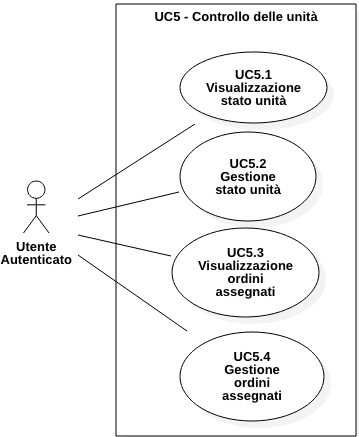
\includegraphics[width=10cm]{images/uc5.png}
    \caption{Diagramma UC5}
\end{figure}
\begin{itemize}
    \item \textbf{Attori primari:} utente autenticato;
    \item \textbf{Descrizione:} l'utente intende visualizzare e/o modificare lo stato e i compiti assegnati delle unità;
    \item \textbf{Scenario principale:} l'utente si trova in un area riservata nella quale viene presentata una lista delle unità collegate al sistema mediante il loro codice identificativo. Grazie ad essa:
    \begin{itemize}
        \item l'utente visualizza lo stato delle unità (UC5.1);
        \item l'utente gestisce lo stato delle unità (UC5.2);
        \item l'utente visualizza la lista di compiti assegnati all'unità (UC5.3);
        \item l'utente gestisce gli ordini assegnati all'unità (UC5.4).
    \end{itemize}
    \item \textbf{Precondizione:} l'utente ha effettuato l'accesso al sistema;
    \item \textbf{Postcondizione:} stato e ordini assegnati dell'unità risultano visualizzati e/o modificati in tempo reale.
\end{itemize}

\subsubsection{UC5.1 - Visualizzazione stato unità}
\begin{itemize}
    \item \textbf{Attori primari:} utente autenticato;
    \item \textbf{Descrizione:} l'utente intende visualizzare lo stato di un'unità;
    \item \textbf{Scenario principale:} l'utente visualizza uno dei possibili stati dell'unità: Start, Stop, Finish, Disconnected.
    \item \textbf{Precondizione:} l'utente ha effettuato l'accesso al sistema;
    \item \textbf{Postcondizione:} l'utente visualizza in tempo reale lo stato dell'unità.
\end{itemize}

\subsubsection{UC5.2 - Gestione stato unità}
\begin{figure}[h!]
    \centering
    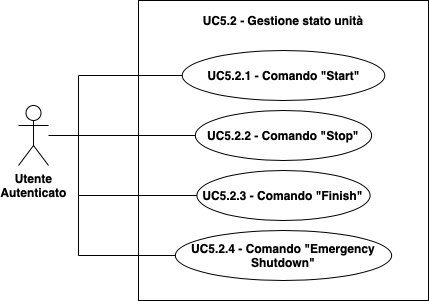
\includegraphics[width=10cm]{images/uc5.2.png}
    \caption{Diagramma UC5.2}
\end{figure}
\begin{itemize}
    \item \textbf{Attori primari:} utente autenticato;
    \item \textbf{Descrizione:} l'utente intende modificare lo stato dell'unità;
    \item \textbf{Scenario principale:} l'utente impartisce determinati comandi per modificare lo stato dell'unità:
    \begin{itemize}
        \item Start (UC5.2.1);
        \item Stop (UC5.2.2);
        \item Finish (UC5.2.3);
        \item Emergency Shutdown (UC5.2.4).
    \end{itemize}
    \item \textbf{Precondizione:} l'unità si trova in un determinato stato.
    \item \textbf{Postcondizione:} l'utente modifica in tempo reale lo stato dell'unità.
\end{itemize}

\subsubsection{UC5.2.1 - Comando "Start"}
\begin{itemize}
    \item \textbf{Attori primari:} utente autenticato;
    \item \textbf{Descrizione:} l'utente intende impostare lo stato dell'unità in modo che consegni tutti gli ordini assegnati eventualmente passando per la base a ritirarli (stato Start);
    \item \textbf{Scenario principale:} l'utente rende Start il nuovo stato dell'unità;
    \item \textbf{Precondizione:} l'unità ha stato Stop o Finish;
    \item \textbf{Postcondizione:} l'unità ha stato Start.
\end{itemize}

\subsubsection{UC5.2.1 - Comando "Stop"}
\begin{itemize}
    \item \textbf{Attori primari:} utente autenticato;
    \item \textbf{Descrizione:} l'utente intende impostare lo stato dell'unità in modo che, pur rimanendo accesa e connessa, si fermi nella posizione attuale (stato Stop);
    \item \textbf{Scenario principale:} l'utente rende Stop il nuovo stato dell'unità;
    \item \textbf{Precondizione:} l'unità ha stato Start o Finish;
    \item \textbf{Postcondizione:} l'unità ha stato Stop.
\end{itemize}

\subsubsection{UC5.2.1 - Comando "Finish"}
\begin{itemize}
    \item \textbf{Attori primari:} utente autenticato;
    \item \textbf{Descrizione:} l'utente intende impostare lo stato dell'unità in modo che consegni gli ordini attualmente assegnati e trasportati per poi rientrare alla base (stato Finish);
    \item \textbf{Scenario principale:} l'utente rende Finish il nuovo stato dell'unità;
    \item \textbf{Precondizione:} l'unità ha stato Start o Stop;
    \item \textbf{Postcondizione:} l'unità ha stato Finish.
\end{itemize}

\subsubsection{UC5.2.1 - Comando "Emergency Shutdown"}
\begin{itemize}
    \item \textbf{Attori primari:} utente autenticato;
    \item \textbf{Descrizione:} l'utente, a causa di un'emergenza, intende spegnere l'unità in modo immediato;
    \item \textbf{Scenario principale:} l'utente spegne l'unità in modo immediato ignorando qualsiasi ordine ancora assegnato;
    \item \textbf{Precondizione:} l'unità ha stato Start, Stop o Finish;
    \item \textbf{Postcondizione:} l'unità è spenta e per il sistema ha stato Disconnected.
\end{itemize}

\subsubsection{UC5.3 - Visualizzazione ordini assegnati}
\begin{itemize}
    \item \textbf{Attori primari:} utente autenticato;
    \item \textbf{Descrizione:} l'utente intende visualizzare la coda degli ordini assegnati;
    \item \textbf{Scenario principale:} l'utente visualizza la coda degli ordini assegnati;
    \item \textbf{Precondizione:} l'utente ha effettuato l'accesso al sistema;
    \item \textbf{Postcondizione:} l'utente visualizza in tempo reale gli ordini assegnati all'unità.
\end{itemize}

\subsubsection{UC5.4 - Gestione ordini assegnati}
\begin{figure}[h!]
    \centering
    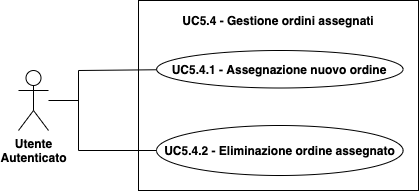
\includegraphics[width=18cm]{images/uc5.4.png}
    \caption{Diagramma UC5.4}
\end{figure}
\begin{itemize}
    \item \textbf{Attori primari:} utente autenticato;
    \item \textbf{Descrizione:} l'utente intende modificare la coda degli ordini assegnati;
    \item \textbf{Scenario principale:} l'utente modifica la coda degli ordini assegnati nei modi seguenti:
    \begin{itemize}
        \item assegnazione nuovo ordine (UC5.4.1);
        \item modifica ordine assegnato (UC5.4.2);
        \item eliminazione ordine assegnato (UC5.4.3).
    \end{itemize}
    \item \textbf{Precondizione:} l'unità ha una coda di ordini;
    \item \textbf{Postcondizione:} la coda degli ordini è modificata.
\end{itemize}

\subsubsection{UC5.4.1 - Assegnazione nuovo ordine}
\begin{itemize}
    \item \textbf{Attori primari:} utente autenticato;
    \item \textbf{Descrizione:} l'utente intende accodare un nuovo ordine;
    \item \textbf{Scenario principale:} l'utente inserisce l'identificativo del POI da visitare per consegnare l'ordine;
    \item \textbf{Estensioni:}
    \begin{itemize}
        \item se l'utente inserisce un POI già presente, viene visualizzato un errore (UC5.4.3);
    \end{itemize}
    \item \textbf{Precondizione:} l'unità ha una coda degli ordini e si trova alla base;
    \item \textbf{Postcondizione:} l'unità ha la precedente coda degli ordini con accodato il nuovo ordine.
\end{itemize}

\subsubsection{UC5.4.2 - Eliminazione ordine assegnato}
\begin{itemize}
    \item \textbf{Attori primari:} utente autenticato;
    \item \textbf{Descrizione:} l'utente intende eliminare un ordine in coda;
    \item \textbf{Scenario principale:} l'utente elimina l'ordine dalla coda indipendentemente dalla sua posizione all'interno di essa;
    \item \textbf{Precondizione:} l'unità ha una coda degli ordini con almeno un elemento e si trova alla base;
    \item \textbf{Postcondizione:} l'unità ha la precedente coda degli ordini con un ordine in meno.
\end{itemize}

\subsubsection{UC5.4.3 - Errore ordine duplicato}
\begin{itemize}
    \item \textbf{Attori primari:} utente autenticato;
    \item \textbf{Descrizione:} l'utente riceve un messaggio d'errore;
    \item \textbf{Scenario principale:} l'utente riceve un messaggio d'errore in cui si segnala che l'ordine è già presente in coda;
    \item \textbf{Precondizione:} l'unità ha una coda degli ordini e si trova alla base;
    \item \textbf{Postcondizione:} viene visualizzato un errore e la coda degli ordini rimane invariata.
\end{itemize}